% !TeX root = ./pf2023.tex

%\includeonlyframes{current}

\section*{Explicit Memory Management\\(Resource Management)}

\begin{frame}{Memory layout of a process}

  \begin{itemize}
  \item A process is a running program
  \item When a program is started the operating system brings the contents of
    the corresponding file into memory according to well-defined conventions
  \end{itemize}

  \begin{columns}
    \begin{column}{.7\textwidth}
      \begin{itemize}
        \item[]
      \begin{itemize}
      \item Stack
        \begin{itemize}
        \item function local variables
        \item function call bookkeeping
        \end{itemize}
      \item Heap
        \begin{itemize}
        \item dynamic allocation
        \end{itemize}
      \item Global data
        \begin{itemize}
        \item literals and variables
        \item initialized and uninitialized (set to 0)
        \end{itemize}
      \item Program instructions
      \end{itemize}
    \end{itemize}
  \end{column}

    \begin{column}{.3\textwidth}
      \centering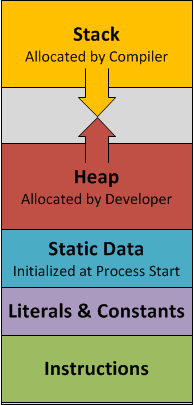
\includegraphics[height=.5\textheight]{images/process-memory-layout}
    \end{column}
  \end{columns}

\end{frame}

\begin{frame}{Dynamic memory allocation}

  \begin{itemize}
  \item<1-> It's not always possible or convenient to construct objects on the
    stack, where they would be destroyed at the end of the function that created
    them
  \item<2-> An object (array of objects) can be constructed on the \textit{free
      store} (\textit{heap})
    \begin{itemize}
    \item \code{new} expression (for an array: \code{new []})
      \begin{itemize}
      \item allocate memory for the object(s)
      \item run the object(s) constructor
      \end{itemize}
    \end{itemize}
  \item<3-> The lifetime of an object (array of objects) on the heap is
    \textbf{explictly} managed by the developer
    \begin{itemize}
    \item explicit destruction of the object(s) when not needed any more
    \item \code{delete} expression (for an array: \code{delete []})
      \begin{itemize}
      \item run the object(s) \textit{destructor} (see later)
      \item deallocate the memory previously allocated for the object(s)
      \end{itemize}
    \end{itemize}
  \item<4-> Contrast this to the \textbf{automatic} destruction of an object at
    the end of the scope when the object is created on the stack
  \end{itemize}

\end{frame}

\begin{frame}[fragile]{Dynamic allocation of an object}

  \begin{columns}[t]
    \begin{column}{.5\textwidth}
      \begin{codeblock}
\visible<2->{auto fun()}
\visible<2->{\{}
\visible<3->{  int n \{1234\};}
\visible<4->{  \visible<7->{int* p =} new int\visible<5->{\{5678\}};}
\visible<8->{  \ddd}
\visible<9->{  delete p;}
\visible<2->{\}}\end{codeblock}

      \begin{itemize}
      \item<10-> \code{delete p} gives the area on the heap back to the system
      \item<11-> \code{delete p} does \textbf{not} modify \code{p}
      \item<12-> After \code{delete p}, the only safe operation on \code{p} is
        an assignment
        \begin{itemize}
        \item \code{p = \ddd;}
        \end{itemize}
      \item<13-> if \code{p} is \code{nullptr}, \code{delete p} is well defined
        and does nothing
      \end{itemize}

    \end{column}

    \begin{column}{.5\textwidth}

      \begin{tikzpicture}[
        mem/.style={
          minimum width=2cm,
          inner sep=0pt,
          outer sep=0pt,
          draw=black
        },
        frame/.style={
          minimum width=2cm,
          inner sep=0pt,
          outer sep=0pt,
          draw=black,
          thick,
          fill=green!50!white
        },
        var/.style={
          node font=\ttfamily\scriptsize,
          minimum height=.5cm,
          minimum width=2cm,
          draw=black,
          fill=green!30!white,
          inner sep=0pt,
          outer sep=0pt
        },
        addr/.style={
          minimum width=0.35cm,
          minimum height=0.5cm,
          draw=black,
          densely dotted
        },
        anchor=south west]

        \visible<1->{
          \node[mem, minimum height=5cm, label={90:Stack}] (stack) {};

          \node[mem, minimum height=5cm, label={90:Heap},right=1cm of stack]
          (heap) {};
        }

        \visible<2->{
          \node[frame,minimum height=1cm,below=0cm of
          stack.north,anchor=north] (funcaller) {};
        }

        \visible<2-9>{
          \node[frame,minimum height=2cm,below=0cm of
          funcaller.south,anchor=north,label={[yshift=.9cm]0:\scriptsize\tt fun}]
          (fun) {};
        }

        \visible<3-9>{
          \node[var,above=.5cm of fun.south,anchor=south,label={180:\scriptsize\tt
            n}] (n) {1234};
        }

        \visible<7-9>{
          \node[var,above=0pt of n,label={180:\scriptsize\tt p}] (p) {0x4ab0};
        }

        \visible<4-8>{
          \node[var,below=2cm of heap.north] (obj) {\only<5->{5678}};
        }

        \visible<6->{
          \node[addr,left=0pt of obj.west,anchor=west,label={270:\tiny\tt 0x4ab0}]
          (objaddr) {};
        }

        \visible<7->{
          \draw[{Circle[length=2pt]}-Stealth] ([xshift=-10pt]p.east) --
          (objaddr.west);
        }
      \end{tikzpicture}

    \end{column}

  \end{columns}

\end{frame}

\begin{frame}[fragile]{Returning a dynamically-allocated object from a function}

  \begin{columns}[t]
    \begin{column}{.45\textwidth}
      \begin{codeblock}
\visible<1->{Sample* create()}
\visible<1->{\{}
\visible<1->{  auto rc = \alert<3>{new Sample\{\}};}
\visible<1->{  rc->add(\ddd);}
\visible<1->{  \ddd}
\visible<1->{  \alert<4>{return rc};}
\visible<1->{\}}

\visible<1->{auto use()}
\visible<1->{\{}
\visible<1->{  auto ru = \alert<2>{create()};}
\visible<1->{  ru->stats();}
\visible<1->{  \ddd}
\visible<1->{  \alert<5>{delete ru};}
\visible<1->{\}}\end{codeblock}

    \end{column}

    \begin{column}{.55\textwidth}

      \begin{tikzpicture}[
        mem/.style={
          minimum width=2cm,
          inner sep=0pt,
          outer sep=0pt,
          draw=black
        },
        frame/.style={
          minimum width=2cm,
          inner sep=0pt,
          outer sep=0pt,
          draw=black,
          thick,
          fill=green!50!white
        },
        var/.style={
          node font=\ttfamily\scriptsize,
          minimum height=.5cm,
          minimum width=2cm,
          draw=black,
          fill=green!30!white,
          inner sep=0pt,
          outer sep=0pt
        },
        addr/.style={
          minimum width=0.35cm,
          minimum height=0.5cm,
          draw=black,
          densely dotted
        },
        anchor=south west]

        \visible<1->{
          \node[mem, minimum height=5cm, label={90:Stack}] (stack) {};

          \node[mem, minimum height=5cm, label={90:Heap},right=1.5cm of stack]
          (heap) {};
        }

        \visible<1->{
          \node[frame,minimum height=1cm,below=0cm of
          stack.north,anchor=north] (caller) {};
        }

        \visible<1-5>{
          \node[frame,minimum height=1.5cm,below=0cm of
          caller.south,anchor=north,label={[yshift=.7cm]0:\scriptsize\tt use}]
          (use) {};
        }

        \visible<2-3>{ \node[frame,minimum height=1.5cm,below=0cm of
          use.south,anchor=north,label={[yshift=.7cm]0:\scriptsize\tt create}]
          (create) {}; }

        \visible<2-3>{
          \node[var,anchor=center,label={180:\scriptsize\tt rc}] at (create)
          (rc) {\only<3>{0xaacc}};
        }

        \visible<1-5>{ \node[var,anchor=center,label={180:\scriptsize\tt ru}] at
          (use) (ru) {\only<4->{0xaacc}}; }

        \visible<3-4>{
          \node[var,minimum height=1.5cm,below=1.3cm of heap.north] (obj) {};
        }

        \visible<3->{
          \node[addr,below left=0pt of obj,anchor=south west,label={270:\tiny\tt 0xaacc}]
          (objaddr) {};
        }

        \visible<3>{
          \draw[{Circle[length=2pt]}-Stealth] ([xshift=-10pt]rc.east) --
          (objaddr.west);
        }

        \visible<4>{
          \draw[{Circle[length=2pt]}-Stealth] ([xshift=-10pt]ru.east) --
          (objaddr.west);
        }
      \end{tikzpicture}

    \end{column}

  \end{columns}

  \vskip 1em

  \uncover<6->{Note how the lifetime of a dynamically-allocated object is
    explicitly managed by the developer}

\end{frame}

\begin{frame}[fragile]{(native) Array of objects}
  Contiguous sequence of homogeneous objects in memory

  \begin{tikzpicture}
    [anchor=south west]
    \visible<2->{\node at (0,0) [
        rectangle,
        draw=black!50,
        minimum width=.9\textwidth,
        minimum height=.5cm,
      ] {};
    }
    \visible<2->{\node at (0,0) [
        rectangle,
        minimum width=0.35cm,
        minimum height=0.5cm,
        draw=black,
        densely dotted,
        label={90:{\scriptsize\tt 0x0000}}
      ] {};
    }
    \visible<2->{\node at (.9\textwidth-.35cm,0) [
        rectangle,
        minimum width=0.35cm,
        minimum height=0.5cm,
        draw=black,
        densely dotted,
        label={90:{\scriptsize\tt 0xffff}}
      ] {};
    }

    \visible<2->{\node at (3.5,0) [
        rectangle,
        fill=green!20!white,
        draw=black!50,
        minimum width=1.5cm,
        minimum height=0.5cm,
        label=270:{\scriptsize\tt\alt<4->{a\alert<4>{[}0\alert<4>{]}}{}},
      ] {\scriptsize\tt\alt<-4|trans:0>{123}{\alert<5|trans:0>{124}}};
    }
    \visible<2->{\node at (5,0) [
        rectangle,
        fill=green!20!white,
        draw=black!50,
        minimum width=1.5cm,
        minimum height=0.5cm,
        label=270:{\scriptsize\tt\alt<4->{a\alert<4>{[}1\alert<4>{]}}{}},
      ] {\scriptsize\tt\alt<-9|trans:0>{456}{\alert<10|trans:0>{654}}};
    }
    \visible<2->{\node at (6.5,0) [
        rectangle,
        fill=green!20!white,
        draw=black!50,
        minimum width=1.5cm,
        minimum height=0.5cm,
        label=270:{\scriptsize\tt\alt<4->{a\alert<4>{[}2\alert<4>{]}}{}},
      ] {\scriptsize\tt 789};
    }

    \visible<2->{\node (addr a0) at (3.5,0) [
        rectangle,
        minimum width=0.35cm,
        minimum height=0.5cm,
        draw=black,
        densely dotted,
        label={90:{\scriptsize\tt\alert<7-8>{0xab00}}}
      ] {};
    }
    \visible<2->{\node (addr a1) at (5,0) [
        rectangle,
        minimum width=0.35cm,
        minimum height=0.5cm,
        draw=black,
        densely dotted,
        label={90:{\scriptsize\tt\alert<9-10>{0xab04}}}
      ] {};
    }
    \visible<2->{\node (addr a2) at (6.5,0) [
        rectangle,
        minimum width=0.35cm,
        minimum height=0.5cm,
        draw=black,
        densely dotted,
        label={90:{\scriptsize\tt 0xab08}}
      ] {};
    }
    \visible<2->{\node (addr a3) at (8,0) [
        rectangle,
        minimum width=0.35cm,
        minimum height=0.5cm,
        draw=black,
        densely dotted,
        label={90:{\scriptsize\tt\alert<11->{0xab0c}}}
      ] {};
    }

    \visible<7->{\node (b) at (1.2,0) [
        rectangle,
        fill=green!20!white,
        draw=black!50,
        minimum width=1.5cm,
        minimum height=0.5cm,
        label=270:{\scriptsize\tt b},
      ] {\scriptsize\tt\alert{\alt<-8|trans:0>{0xab00}{\alt<-10|trans:0>{0xab04}{0xab0c}}}};
    }
    \visible<7->{\node at (1.2,0) [
        rectangle,
        minimum width=0.35cm,
        minimum height=0.5cm,
        draw=black,
        densely dotted,
        label={90:{\scriptsize\tt 0xaa00}}
      ] {};
    }

    \draw<7-8>[{Circle[length=2pt]}-Stealth,opacity=.6] ([yshift=.1cm]b.center) .. controls +(1.5,.5) .. (addr a0.north);
    \draw<9-10>[{Circle[length=2pt]}-Stealth,opacity=.6] ([yshift=.1cm]b.center) .. controls +(3,.5) .. (addr a1.north);
    \draw<11->[{Circle[length=2pt]}-Stealth,opacity=.6] ([yshift=.1cm]b.center) .. controls +(6,.5) .. (addr a3.north);

  \end{tikzpicture}

  \begin{codeblock}<3->{
\uncover<3->{int a[3] = \{123, 456, 789\}; // int[3], the size must be a constant
                            // and can be deduced from the initializer}
\uncover<5->{++a\alert<5>{[}0\alert<5>{]};}
\uncover<6->{a[3];                       // undefined behavior}
\uncover<7->{// "arrays decay to pointers at the slightest provocation"
auto b = a;                 // int*, size information lost}
\uncover<8->{assert(b == &a[0]);}
\uncover<9->{++b;                        // increase by sizeof(int)
assert(b == &a[1]);}
\uncover<10->{*b = 654;}
\uncover<11->{b += 2;                     // increase by 2 * sizeof(int)}
\uncover<12->{*b;                         // undefined behavior}
\uncover<13->{if (b == a + 3) \{ ... \}     // ok, but not more than this}}\end{codeblock}

\end{frame}

\begin{frame}[fragile]{Dynamic allocation of an array of objects}

  \begin{columns}
    \begin{column}{.5\textwidth}
      \begin{codeblock}
\visible<2->{auto fun()}
\visible<2->{\{}
\visible<3->{  int a[3] \{12, 34, 56\};}
\visible<4->{  \visible<7->{\alt<-7|trans:0>{auto}{\alert<8|trans:0>{int*}} p =} new int[3] \visible<5->{\{12, 34, 56\}};}
\visible<9->{  \ddd}
\visible<10->{  delete [] p;}
\visible<2->{\}}\end{codeblock}

      \begin{itemize}
      \item<11-> \code{p} points to the first element of the array
      \item<12-> \code{p} does \textbf{not} carry ``array'' information
      \end{itemize}

    \end{column}

    \begin{column}{.5\textwidth}

      \begin{tikzpicture}[
        mem/.style={
          minimum width=2cm,
          inner sep=0pt,
          outer sep=0pt,
          draw=black
        },
        frame/.style={
          minimum width=2cm,
          inner sep=0pt,
          outer sep=0pt,
          draw=black,
          thick,
          fill=green!50!white
        },
        var/.style={
          node font=\ttfamily\scriptsize,
          minimum height=.5cm,
          minimum width=2cm,
          draw=black,
          fill=green!30!white,
          inner sep=0pt,
          outer sep=0pt
        },
        addr/.style={
          minimum width=0.35cm,
          minimum height=0.5cm,
          draw=black,
          densely dotted
        },
        anchor=south west]

        \visible<1->{
          \node[mem, minimum height=7cm, label={90:Stack}] (stack) {};

          \node[mem, minimum height=7cm, label={90:Heap},right=1cm of stack]
          (heap) {};
        }

        \visible<2->{
          \node[frame,minimum height=3cm,below=0cm of
          stack.north,anchor=north] (funcaller) {};
        }

        \visible<2-10>{
          \node[frame,minimum height=3cm,below=0cm of
          funcaller.south,anchor=north,label={[yshift=1.2cm]0:\scriptsize\tt fun}]
          (fun) {};
        }

        \visible<3-10>{
          \node[var,above=.5cm of fun.south,anchor=south,label={180:\scriptsize\tt
            a[0]}] (a0) {12};
          \node[var,above=0pt of a0,anchor=south,label={180:\scriptsize\tt
            a[1]}] (a1) {34};
          \node[var,above=0pt of a1,anchor=south,label={180:\scriptsize\tt
            a[2]}] (a2) {56};
        }

        \visible<7-10>{
          \node[var,above=0pt of a2,label={180:\scriptsize\tt p}] (p) {0xed80};
        }

        \visible<4-9>{
          \node[var,below=2cm of heap.north,label={180:\only<9->{\scriptsize\tt p[0]}}]
          (p0) {\only<5->{12}};
          \node[var,above=0pt of p0,label={180:\only<9->{\scriptsize\tt p[1]}}] (p1)
          {\only<5->{34}};
          \node[var,above=0pt of p1,label={180:\only<9->{\scriptsize\tt p[2]}}] (p2)
          {\only<5->{56}};
        }

        \visible<6->{
          \node[addr,left=0pt of p0.west,anchor=west,label={270:\tiny\tt 0xed80}]
          (p0addr) {};
        }

        \visible<7->{
          \draw[{Circle[length=2pt]}-Stealth] ([xshift=-10pt]p.east) --
          (p0addr.west);
        }
      \end{tikzpicture}

    \end{column}

  \end{columns}

\end{frame}

\begin{frame}[fragile]{Dynamic allocation of an array of objects of dynamic size}

  Arrays allocated on the heap are most useful when their size is available only
  at runtime

  \begin{columns}[t]
    \begin{column}{.4\textwidth}
      \begin{codeblock}<2->{
auto fun()
\{
  int n;
  std::cin >> n;
  auto p = new int[n];
  \ddd
  delete [] p;
\}}\end{codeblock}

    \end{column}

    \begin{column}{.6\textwidth}

      \visible<3->{
        \begin{tikzpicture}[
          mem/.style={
            minimum width=2cm,
            inner sep=0pt,
            outer sep=0pt,
            draw=black
          },
          frame/.style={
            minimum width=2cm,
            inner sep=0pt,
            outer sep=0pt,
            draw=black,
            thick,
            fill=green!50!white
          },
          var/.style={
            node font=\ttfamily\scriptsize,
            minimum height=.5cm,
            minimum width=2cm,
            draw=black,
            fill=green!30!white,
            inner sep=0pt,
            outer sep=0pt
          },
          addr/.style={
            minimum width=0.35cm,
            minimum height=0.5cm,
            draw=black,
            densely dotted
          },
          anchor=south west]

          \node[mem, minimum height=5cm, label={90:Stack}] (stack) {};

          \node[mem, minimum height=5cm, label={90:Heap},right=2cm of stack]
          (heap) {};

          \node[frame,minimum height=1cm,below=0cm of stack.north,anchor=north]
          (funcaller) {};

          \node[frame,minimum height=2cm,below=0cm of
          funcaller.south,anchor=north,label={[yshift=.5cm]0:\scriptsize\tt fun}]
          (fun) {};

          \node[var,above=.5cm of fun.south,anchor=south,label={180:\scriptsize\tt
            n}] (n) {\ddd};

          \node[var,above=.0pt of n.north,anchor=south,label={180:\scriptsize\tt
            p}] (p) {0xc408};

          \node[var,below=3cm of heap.north,label={180:\scriptsize\tt p[0]}] (p0)
          {};

          \node[var,above=0pt of p0,label={180:\scriptsize\tt p[1]}] (p1) {};

          \node[var,minimum height=1.5cm,above=0pt of p1,label={180:$\vdots$}]
          (pi) {$\vdots$};

          \node[var,above=0pt of pi,label={180:\scriptsize\tt p[n-1]}]
          (pnminus1) {};

          \node[addr,left=0pt of p0.west,anchor=west,label={270:\tiny\tt 0xc408}]
          (p0addr) {};

          \draw[{Circle[length=2pt]}-Stealth] ([xshift=-10pt]p.east) --
          (p0addr.west);
        \end{tikzpicture}
      }
    \end{column}

  \end{columns}

\end{frame}

\begin{frame}{Null-terminated byte strings}
  \begin{itemize}
  \item<1-> A null-terminated byte string (NTBS) is an array of non-null characters
    followed by the null character (\code{char\{0\}} or \code{\bslashz})
    \begin{itemize}
    \item \code{char[]} (\code{char*}) if characters are modifiable
    \item \code{char const[]} (\code{char const*}) if characters are not
      modifiable
    \item Also known as ``C-strings''
    \end{itemize}
  \item<2-> The \code{std::strlen} function returns the length of an NTBS
    \begin{itemize}
    \item Linear complexity, scan the array until \code{\bslashz} is found
    \end{itemize}
  \item<3-> A string literal has type \code{char const[N]}, with \code{N} constant
    \begin{itemize}
    \item For example, the type of \code{"ciao"} is \code{char const[5]}
    \end{itemize}
  \item<4-> An \code{std::string} can be initialized with an NTBS
  \item<4-> To get the NTBS representation of an \code{std::string} use the
    \code{c_str} method
    \begin{itemize}
    \item It returns a \code{char const*} to the internal array
    \end{itemize}
  \end{itemize}

\end{frame}

\begin{frame}{The \code{main} function}
  \begin{itemize}
  \item The \code{main} (special) function is the entry point of a program
  \item It can have two forms
    \begin{itemize}
    \item \code{int main() \{\ddd\}}
    \item \code{int main(int argc, char* argv[]) \{\ddd\}}
    \end{itemize}
  \item If there is no \code{return} statement, an implicit \code{return 0;} is assumed
    \begin{itemize}
    \item $0$ means success, different from $0$ means failure
    \end{itemize}
  \item \code{argc} is the number of arguments on the command line, \code{argv}
    is an array of C-strings representing the arguments
    \begin{itemize}
    \item \code{argv[0]} is (usually) the name of the program
    \item \code{argv[argc]} is \code{nullptr}
    \end{itemize}
  \item Many libraries exist to parse the command line, e.g.
    \href{https://github.com/bfgroup/Lyra}{Lyra},
    \href{https://github.com/jarro2783/cxxopts}{cxxopts},
    \href{https://www.boost.org/doc/libs/release/libs/program_options/}{Boost.Program_options}
  \end{itemize}
\end{frame}

\begin{frame}{Managing raw arrays}

  \begin{itemize}
  \item Managing raw arrays \textbf{correctly} is difficult
  \item Passing an array around makes it decay to a pointer to its first
    element, loosing important type information
  \item How do you pass an array to a function?
    \begin{itemize}
    \item Need to pass pointer and size
    \item \Cpp{}20 introduces \code{std::span}
    \end{itemize}
  \item How do you return an array from a function?
    \begin{itemize}
    \item Left as an exercise
    \end{itemize}
  \item Better use higher-level tools, such as \code{std::string},
    \code{std::array} and \code{std::vector}
  \end{itemize}
\end{frame}

\begin{frame}[fragile]{Weaknesses of a \code{T*}}

  \begin{itemize}
  \item<1-> Critical information is not encoded in the type
    \begin{itemize}
    \item<2-> Am I the owner of the pointee? Should I delete it?
      \begin{codeblock}<2->{
Shape* s = create_shape();               // (probably) delete

\visible<3->{std::string str\{"hello"\};
char const* cs = str.c_str();            // don\textquotesingle{}t delete
char      * cd = str.data();             // don\textquotesingle{}t delete, const is irrelevant}}\end{codeblock}

    \item<4-> Is the pointee an object or an array of objects? of what size?
      \begin{codeblock}<4->{
Shape* s = create_shape\textbf{s}();               // (probably) delete \textbf{[]}}\end{codeblock}

    \item<5-> Was it allocated with \code{new}, \code{malloc} or even something
      else?
      \begin{itemize}
      \item \code{malloc} is a C function that allocates raw memory, which is
        then de-allocated passing the pointer to the function \code{free}
      \item e.g. the \code{fopen} function returns a \code{FILE*}, which will be
        released passing it to the \code{fclose} function
      \end{itemize}

    \end{itemize}
  \end{itemize}
\end{frame}

\begin{frame}[fragile]{Weaknesses of a \code{T*} \insertcontinuationtext}

  \begin{itemize}
  \item Owning pointers are prone to leaks
    \begin{codeblock}
\{
  auto p = new Circle\{\ddd\};
  \ddd
  // ops, forgot to delete p
\}\end{codeblock}

  \item<2-> Owning pointers are prone to double \code{delete}s
    \begin{codeblock}
\{
  auto p = new Circle\{\ddd\};
  \ddd
  delete p;
  \ddd
  delete p; // ops, delete again
\}\end{codeblock}

  \end{itemize}
\end{frame}

\begin{frame}[fragile]{Weaknesses of a \code{T*} \insertcontinuationtext}

  \begin{itemize}
  \item<1-> Owning pointers are unsafe in presence of exceptions
    \begin{codeblock}
\{
  auto p = new Circle\{\ddd\};
  \ddd                         // potentially throwing code
  delete p;                  // leak if exception thrown
\}\end{codeblock}

  \item<2-> Runtime overhead, in space and time
    \begin{itemize}
    \item dynamic allocation/deallocation
    \item indirection
    \end{itemize}
  \end{itemize}

\end{frame}

\begin{frame}[fragile]{Stack vs Heap: space}

  \begin{columns}[T]
    \begin{column}{.3\textwidth}

  \begin{codeblock}{
struct S \{
  int    n;
  float  f;
  double d;
\};

\uncover<2->{auto foo_s() \{
  S s;
  \ddd
\}}

\uncover<4->{auto foo_h() \{
  S* s = new S;
  \ddd
\}}}\end{codeblock}
    \end{column}

    \setlength{\bytesize}{0.2cm}
    \setlength{\memwidth}{8\bytesize}
    \setlength{\memheight}{5cm}

    \begin{column}{.3\textwidth}
      \uncover<2->{\begin{tikzpicture}
        [anchor=south west]
        \node (memory) at (0,0) [
          rectangle,
          minimum width=\memwidth,
          minimum height=\memheight,
          draw=black
        ] {};
        \node at (0,3) [
          rectangle,
          minimum width=\memwidth,
          minimum height=5\bytesize,
          draw=black,
          fill=green!30!white,
          label={[yshift=-.4cm]\scriptsize\tt foo\_s}
        ] {};
        \node at (0,4) [
          rectangle,
          minimum width=\memwidth,
          minimum height=1cm,
          draw=black,
          fill=green!10!white
        ] {};
        \node at (0,3.1) [
          rectangle,
          minimum width=.5\memwidth,
          minimum height=\bytesize,
          draw=black,
          fill=red
        ] {};
        \node at (.5\memwidth,3.1) [
          rectangle,
          minimum width=.5\memwidth,
          minimum height=\bytesize,
          draw=black,
          fill=blue
        ] {};
        \node at (0,3.1cm + \bytesize) [
          rectangle,
          minimum width=\memwidth,
          minimum height=\bytesize,
          draw=black,
          fill=yellow
        ] {};
        \node at (0,0) [
          rectangle,
          inner sep=0pt,
          minimum width=\bytesize,
          minimum height=\bytesize,
          draw=black,
          densely dotted,
          label={270:{\tiny\tt 0x00..00}}
        ] {};
        \node at (\memwidth-\bytesize,\memheight-\bytesize) [
          rectangle,
          inner sep=0pt,
          minimum width=\bytesize,
          minimum height=\bytesize,
          draw=black,
          densely dotted,
          label={90:{\tiny\tt 0xff..ff}}
        ] {};
        \draw [dashed] (-.5cm,.5\memheight) -- (\memwidth + .5cm,.5\memheight);
        \node at (0,4) [rotate=90] {\scriptsize\textit{stack}};
        \node at (0,0) [rotate=90] {\scriptsize\textit{heap}};
      \end{tikzpicture}}

      \uncover<3->{\scriptsize Occupancy:
      \begin{itemize}
      \item \code{sizeof(S)}
      \end{itemize}}

    \end{column}

    \begin{column}{.3\textwidth}

      \uncover<4->{\begin{tikzpicture}
        [anchor=south west]
        \node (memory) at (0,0) [
          rectangle,
          minimum width=\memwidth,
          minimum height=\memheight,
          draw=black
        ] {};
        \node at (0,3) [
          rectangle,
          minimum width=\memwidth,
          minimum height=5\bytesize,
          draw=black,
          fill=green!30!white,
          label={[yshift=-.4cm]\scriptsize\tt foo\_h}
        ] {};
        \node at (0,4) [
          rectangle,
          minimum width=\memwidth,
          minimum height=1cm,
          draw=black,
          fill=green!10!white
        ] {};
        \node (ptr) at (0,3.1cm) [
          rectangle,
          minimum width=\memwidth,
          minimum height=\bytesize,
          draw=black,
          fill=green
        ] {};
        \node (alloc) at (0,1.1) [
          rectangle,
          minimum width=.5\memwidth,
          minimum height=\bytesize,
          draw=black,
          fill=red
        ] {};
        \node at (.5\memwidth,1.1) [
          rectangle,
          minimum width=.5\memwidth,
          minimum height=\bytesize,
          draw=black,
          fill=blue
        ] {};
        \node at (0,1.1cm + \bytesize) [
          rectangle,
          minimum width=\memwidth,
          minimum height=\bytesize,
          draw=black,
          fill=yellow
        ] {};
        \draw[{Circle[length=2pt]}-Stealth,opacity=.6] (ptr.center) .. controls +(-1.5,-1) .. (alloc.base west);
        \node at (0,0) [
          rectangle,
          inner sep=0pt,
          minimum width=\bytesize,
          minimum height=\bytesize,
          draw=black,
          densely dotted,
          label={270:{\tiny\tt 0x00..00}}
        ] {};
        \node at (\memwidth-\bytesize,\memheight-\bytesize) [
          rectangle,
          inner sep=0pt,
          minimum width=\bytesize,
          minimum height=\bytesize,
          draw=black,
          densely dotted,
          label={90:{\tiny\tt 0xff..ff}}
        ] {};
        \draw [dashed] (-.5cm,.5\memheight) -- (\memwidth + .5cm,.5\memheight);
        \node at (0,4) [rotate=90] {\scriptsize\textit{stack}};
        \node at (0,0) [rotate=90] {\scriptsize\textit{heap}};
      \end{tikzpicture}}

      \uncover<5->{\scriptsize Occupancy:
      \begin{itemize}
      \item \code{sizeof(S)} + \code{sizeof(S*)}
      \item plus \code{new} internal space overhead
      \end{itemize}}

    \end{column}
  \end{columns}
\end{frame}

\begin{frame}[fragile]{Stack vs Heap: time}
  \begin{columns}[T]
    \begin{column}{.4\textwidth}
      Stack
      \begin{codeblock}{\tiny
void stack()
\{
  int m\{123\};
  \ddd
\}}\end{codeblock}
      \begin{codeblock}<2->{\tiny
stack():
     subq %4, %rsp
     movl $123, (%rsp)
     \ddd
     addq $4, %rsp
     ret}\end{codeblock}
    \end{column}

    \begin{column}{.6\textwidth}
      Heap
      \begin{codeblock}{\tiny
void heap()
\{
  int* m = new int\{123\};
  \ddd
  delete m;
\}}\end{codeblock}
      \begin{codeblock}<3->{\tiny
heap():
     subq	$8, %rsp
     movl	$4, %edi
     \alert{call	operator new(unsigned long)}
     movl	$123, (%rax)
     movq %rax, (%rsp)
     \ddd
     movl	$4, %esi
     movq	%rax, %rdi
     \alert{call	operator delete(void*, unsigned long)}
     addq	$8, %rsp
     ret}\end{codeblock}
      \begin{codeblock}<4->{\tiny
$ g++ -O3 heap.cpp && ./a.out
1000000 iterations: 0.035745 s}\end{codeblock}

\uncover<4->{\scriptsize i.e. \~35 ns for each \code{new}/\code{delete} (on my
  laptop)}

    \end{column}
  \end{columns}
\end{frame}

\begin{frame}[fragile]{Investigating memory problems}

  \begin{itemize}
  \item One of the simplest tools to use is the \textit{Address Sanitizer}
    (ASan)
  \item The compiler instruments the executable so that at runtime ASan can
    catch many (but not all!) memory problems
  \item Some space and time overhead at runtime, but acceptable at least during
    testing
  \end{itemize}

    \begin{shellblock}<2->{
$ g++ -fsanitize=address leak.cpp
$ ./a.out

=================================================================
==18338==ERROR: LeakSanitizer: detected memory leaks
\ldots}\end{shellblock}

\end{frame}

\begin{frame}{Guidelines on dynamic objects}

  \begin{itemize}
  \item Do not unnecessarily allocate on the heap, i.e. use the stack when
    possible
  \item If unavoidable, think thoroughly about ownership and use a
    resource-managing object, e.g.
    \begin{itemize}
    \item containers and strings
    \item \textit{smart pointers} (see later)
    \end{itemize}
  \item Ideally the residual meaning of a raw pointer (\code{T*}) should be
    ``I'm pointing to \textbf{one} element and I'm \textbf{not} its owner''
  \end{itemize}
\end{frame}

\begin{frame}{Resource management}
  \begin{itemize}
  \item<1-> Dynamic memory is just one of the many types of resources manipulated by a
    program:
    \begin{itemize}
    \item thread, mutex, socket, file, \ldots
    \end{itemize}
  \item<2-> C++ offers powerful tools to manage resources
    \begin{itemize}
    \item \textit{"C++ is my favorite garbage collected language because it
      generates so little garbage"}
    \end{itemize}
  \end{itemize}

\end{frame}

\begin{frame}[fragile]{Destruction}

  \begin{itemize}
  \item<1-> At the end of a block statement (i.e. when the closing brace
    \alert{\}} is encountered) all objects of automatic storage duration are
    automatically \textit{destroyed}
  \item<2-> Destroying an object means
    \begin{itemize}
    \item for a class type, a special member function, called
      \textit{destructor}, if present, is run
    \item all the sub-objects (e.g. data members) are destroyed, recursively
    \item the storage is freed
    \end{itemize}
  \item<3-> The order of destruction is the opposite of the order of
    construction/definition
    \begin{itemize}
    \item a later-defined object can use a previously-defined one
    \end{itemize}
  \end{itemize}

  \begin{codeblock}<3->{
\{
  S s\{\ddd\};
  \ddd
  T t\{s\};
  \ddd
\} // t is destroyed first, then s}\end{codeblock}

\end{frame}

\begin{frame}[fragile]{The destructor}

  \begin{itemize}[<+->]
  \item The \textit{destructor} is a special class member function that is
    called when an object of that class goes out of scope and has to be
    destroyed
  \item The purpose of the destructor is to leave no garbage behind
  \item A class can have only one destructor, declared as
    \code{\~\textit{classname}()}
  \end{itemize}

  \begin{codeblock}<+->{
class DynamicArray \{
  \ddd
  int* m_data;
 public:
  DynamicArray(int n): m_data\{new int[n]\} \{\ddd\}
  ~DynamicArray()
  \{
    delete [] m_data;
  \}
  \ddd
\};
}\end{codeblock}

\end{frame}

\begin{frame}{RAII idiom}

  \begin{itemize}[<+->]
  \item Resource Acquisition Is Initialization
    \begin{itemize}
    \item The constructor accepts/acquires a resource
    \item The destructor releases it
    \end{itemize}
  \item The object is responsible for the correct lifetime management of that
    resource
  \item Guaranteed no leak nor double release, even in presence of exceptions
  \end{itemize}

\end{frame}

\begin{frame}[fragile]{Controlling copying}
  \begin{itemize}
  \item<1-> The compiler automatically generates the copy operations for a class, if used
    \begin{itemize}
    \item The copy constructor creates a \alert{new} object as a copy of
      another object

      \begin{codeblock}
DynamicArray original\{\ddd\};
auto copy\{original\}; // auto copy = original\end{codeblock}

    \item The copy assignment operator changes the value of an \alert{existing}
      object as a copy of another object

      \begin{codeblock}
DynamicArray v1\{\ddd\};
DynamicArray v2\{\ddd\};
v2 = v1;\end{codeblock}

    \end{itemize}

  \item<2-> Ideally, after a copy the two objects should compare equal
  \item<3-> The generated operations may not be correct, especially in presence of
    managed resources (e.g. dynamically-allocated memory)
  \item<3-> The copy operations can be explicitly provided or suppressed
  \end{itemize}
\end{frame}

\begin{frame}[fragile]{Controlling copying \insertcontinuationtext}

  \begin{itemize}
  \item The copy constructor typically takes an object of the same class by
    const reference
    \begin{codeblock}
DynamicArray(DynamicArray const& other) : \ddd \{\ddd\}\end{codeblock}

  \item The copy assignment operator typically:
    \begin{itemize}
    \item takes an object of the same class by const reference
    \item returns the object itself by reference
    \item checks for auto-assignment
    \end{itemize}

    \begin{codeblock}
DynamicArray& operator=(DynamicArray const& other)
\{
  if (this != &other) \{
    \ddd
  \}
  return *this;
\}\end{codeblock}

  \end{itemize}
\end{frame}

\begin{frame}[fragile]{Controlling copying \insertcontinuationtext}
    \begin{codeblock}
class DynamicArray
\{
  int m_size = 0; int* m_data = nullptr;
 public:
  DynamicArray(int n, int v = int\{\}) : m_size\{n\}, m_data\{new int[m_size]\}
  \{ std::fill(m_data, m_data + m_size, v); \}
  ~DynamicArray() \{ delete[] m_data; \}
  \alert{DynamicArray(DynamicArray const& other)}
      : m_size\{other.m_size\}, m_data\{new int[m_size]\}
  \{ std::copy(other.m_data, other.m_data + m_size, m_data); \}
  \alert{DynamicArray& operator=(DynamicArray const& other)}
  \{
    if (this != &other) \{
      delete[] m_data;
      m_size = other.m_size;
      m_data = new int[m_size];
      std::copy(other.m_data, other.m_data + m_size, m_data);
    \}
    return *this;
  \}
  \ddd
\};\end{codeblock}

\end{frame}

\begin{frame}{Smart pointers}
  \begin{itemize}
  \item A \textit{smart pointer} is an object that behaves like a pointer, but
    also manages the lifetime of the pointed-to object (i.e. the pointee)
  \item It leverages the RAII idiom
    \begin{itemize}
    \item Resource Acquisition Is Initialization
    \item Resource (e.g. memory) is acquired in the constructor
    \item Resource (e.g. memory) is released in the destructor
    \end{itemize}
  \end{itemize}
\end{frame}

\begin{frame}[fragile]{Smart pointers \insertcontinuationtext}
  \begin{codeblock}
template<typename Pointee>
class SmartPointer \{
  Pointee* m_p;
 public:
  explicit SmartPointer(Pointee* p): m_p\{p\} \{\}
  \alert<2>{~SmartPointer() \{ delete m_p; \}}
  \visible<4->{Pointee* operator\alert<4>{->}() \{ return m_p; \}
  Pointee& operator\alert<4>{*}() \{ return *m_p; \}}
\};

class Sample \{ \ddd \};

\{
  SmartPointer<Sample> \alert<2>{sp}\{new Sample\{\}\};
  \visible<3->{sp\alert<3-4>{->}add(\ddd);
  (\alert<3-4>{*}sp).stats();}
\alert<2>{\}}\end{codeblock}

\uncover<2->{At the end of the scope (i.e. at the closing \code{\}}) \code{sp}
  is destroyed and its destructor \code{delete}s the pointee}

\end{frame}

\begin{frame}[fragile]{\code{std::unique_ptr<T>}}

  Standard smart pointer

  \begin{itemize}
  \item Exclusive ownership
  \item Minimal overhead, if any
  \item Non-copyable, movable
  \end{itemize}

  \begin{codeblock}<2->{
class Sample \{ \ddd \};

void take(std::unique_ptr<Sample> q); \uncover<6->{       \alert<6>{// by value}}

\uncover<3->{std::unique_ptr<Sample> p\{new Sample\{\}\}; // explicit new}
\uncover<4->{auto p = std::make_unique<Sample>();     // better (*)}
\uncover<5->{auto r = p;}                              \uncover<6->{// error, non-copyable}
\uncover<5->{take(p);}                                 \uncover<6->{// error, non-copyable}
\uncover<7->{auto r = \alert<7>{std::move(}p\alert<7>{)};}                   \uncover<8->{// ok, movable}
\uncover<7->{take(\alert<7>{std::move(}r\alert<7>{)});}                      \uncover<8->{// ok, movable}}\end{codeblock}

  \uncover<4->{(*) The possible arguments passed to \code{make_unique} are
    \textit{forwarded} to the constructor}
\end{frame}

\begin{frame}[fragile]{Disabling copy operations}
  \begin{itemize}
  \item<1-> If a class cannot support copy semantics, its copy operations should be
    suppressed
  \item<2-> The cleanest way to do it is to mark the copy operations as
    \code{=~delete}
    \begin{codeblock}<3->
template<typename Pointee>
class UniquePtr \{
  Pointee* m_p;
 public:
  explicit UniquePtr(Pointee* p): m_p\{p\} \{\}
  ~UniquePtr() \{ delete m_p; \}
  UniquePtr(UniquePtr const&) \alert{= delete};
  UniquePtr& operator=(UniquePtr const&) \alert{= delete};
  Pointee* operator->() \{ return m_p; \}
  Pointee& operator*() \{ return *m_p; \}
\};\end{codeblock}

  \item<4-> Note that a deleted copy ctor is still a ctor and would disable the
  generation of the default ctor
  \item<5-> \code{=~delete} is a general mechanism that can be applied to any
    function
  \end{itemize}
\end{frame}

\begin{frame}{Move semantics}

  \begin{itemize}
  \item It allows to properly \textit{move} (i.e. pass) the responsibility of a
    resource from one managing object to another
  \item Mainly driven by optimization considerations but also a solution to
    a proper management of resources
  \item Introduced in the language by \Cpp{}11, thanks to a new type of reference,
    called \textit{rvalue reference}
  \item An \textit{rvalue reference} is identified by the token \code{\&\&}, e.g.
    \code{int\&\&}
  \end{itemize}

\end{frame}

\begin{frame}[fragile]{Controlling moving}
  \begin{itemize}
  \item<1-> The compiler automatically generates the move operations for a class, if
    used
    \begin{itemize}
    \item The move constructor creates a \alert{new} object, \alert{re-using} the
      resources owned by another object

      \begin{codeblock}
UniquePtr<int> p\{new int\{42\}\};
auto q\{std::move(p)\}; // auto q = std::move(p)\end{codeblock}

     \item The move assignment operator changes the value of an \alert{existing}
       object, \alert{re-using} the resources owned by another object

      \begin{codeblock}
UniquePtr<int> p\{new int\{12\}\};
UniquePtr<int> q\{new int\{34\}\};
q = std::move(p);\end{codeblock}

     \end{itemize}
   \item<2-> \code{std::move} enables the use of a move operation instead of the
     corresponding copy operation
     \begin{itemize}
     \item In practice it's a \code{static_cast} of an lvalue reference to an
       rvalue reference
     \end{itemize}
  \end{itemize}
\end{frame}

\begin{frame}{Controlling moving \insertcontinuationtext}

  \begin{itemize}
  \item<1-> If there are no resources involved, a move operation in fact becomes
    a copy operation
  \item<2-> Move operations typically modify the source object, to steal its
    internal resources
  \item<2-> After a move the two objects are typically different
  \item<3-> A move should leave the original object in a \textit{``valid but
      unspecified state''}
    \begin{itemize}
    \item i.e. \textbf{the class invariant is preserved}
    \item not always easy, especially for the move constructor
    \end{itemize}
  \item<4-> Move operations should be declared \code{noexcept}, which means
    ``this function/operation doesn't fail'' (more or less)
  \item<5-> The automatically generated operations may not be correct
  \item<5-> The move operations can be explicitly provided or suppressed
  \end{itemize}

\end{frame}

\begin{frame}[fragile]{Controlling moving \insertcontinuationtext}
  \begin{codeblock}
template <typename Pointee> class UniquePtr
\{
  Pointee* m_p;
 public:
  explicit UniquePtr(Pointee* p = nullptr) : m_p{p} \{\}
  ~UniquePtr() \{ delete m_p; \}
  UniquePtr(UniquePtr const&) = delete;
  UniquePtr& operator=(UniquePtr const&) = delete;
  \alert{UniquePtr(UniquePtr&& other)} noexcept
      : m_p\{std::exchange(other.m_p, nullptr)\}
  \{
  \}
  \alert{UniquePtr& operator=(UniquePtr&& other)} noexcept
  \{
    delete m_p;
    m_p = std::exchange(other.m_p, nullptr);
    return *this;
  \}
  \ddd
\};\end{codeblock}

\end{frame}

\begin{frame}[fragile]{Controlling moving \insertcontinuationtext}

  \begin{itemize}
  \item The move constructor typically takes an object of the same class by
    (non-const!) rvalue reference
    \begin{codeblock}
UniquePtr(UniquePtrs&& other) : \ddd \{\ddd\}\end{codeblock}

  \item The move assignment operator typically:
    \begin{itemize}
    \item takes an object of the same class by (non-const) rvalue reference
    \item returns the object itself by reference
    \item does \textbf{not} check for auto-assignment
    \end{itemize}

    \begin{codeblock}
UniquePtr& operator=(UniquePtr&& other)
\{
  \ddd
  return *this;
\}\end{codeblock}

  \end{itemize}
\end{frame}

\begin{frame}[fragile]{Special member functions}
  \begin{itemize}
  \item A class has five special member functions
    \begin{itemize}
    \item Plus the default constructor
    \end{itemize}

    \begin{codeblock}
class MyClass \{
  MyClass(MyClass const&);            // copy constructor
  MyClass& operator=(MyClass const&); // copy assignment
  MyClass(MyClass&&);                 // move constructor
  MyClass& operator=(MyClass&&);      // move assignment
  ~MyClass();                         // destructor
\};\end{codeblock}

  \item<2-> The compiler can generate them automatically according to some
    convoluted rules
    \begin{itemize}
    \item The behavior depends on the behavior of data members
    \end{itemize}
  \item<3-> General guidelines:
    \begin{description}
    \item [Rule of zero] Don't declare them and rely on the compiler
    \item [Rule of five] If you need to declare one, declare them all
    \end{description}
    \begin{itemize}
    \item Consider using \code{=default} and \code{=delete}
    \end{itemize}
  \end{itemize}

\end{frame}

\begin{frame}[fragile]{\code{std::shared_ptr<T>}}

  Standard smart pointer

  \begin{itemize}
  \item Shared ownership (reference counted)
  \item Some space and time overhead
    \begin{itemize}
    \item for the management, not for access
    \end{itemize}
  \item Copyable and movable
  \end{itemize}

  \begin{codeblock}<2->{
class Sample \{ \ddd \};

void take(std::shared_ptr<Sample> q);        // by value

\uncover<3->{std::shared_ptr<Sample> p\{new Sample\{\}\};     // explicit new}
\uncover<4->{auto p = std::make_shared<Sample>();         // better (*)}
\uncover<5->{auto s = p;}                                 \uncover<6->{// ok, copyable}
\uncover<5->{take(p);}                                    \uncover<6->{// ok, copyable}
\uncover<7->{auto s = std::move(p);}                      \uncover<8->{// ok, movable}
\uncover<7->{take(std::move(s));}                         \uncover<8->{// ok, movable}}\end{codeblock}

  \uncover<4->{(*) The possible arguments passed to \code{make_shared} are
    \textit{forwarded} to the constructor}

\end{frame}

\begin{frame}[fragile]{Using smart pointers}

    \begin{itemize}[<+->]

    \item Give an owning raw pointer (e.g. the result of a call to \code{new})
      to a smart pointer as soon as possible
    \item Prefer \code{unique_ptr} unless you need \code{shared_ptr}
      \begin{itemize}[<.->]
      \item You can always move a \code{unique_ptr} into a \code{shared_ptr}
      \item But not viceversa
      \end{itemize}

    \item Access to the raw pointer is available
      \begin{itemize}[<.->]
      \item e.g. to pass to legacy APIs
      \item \code{\textit{smart}_ptr<T>::get()}
        \begin{itemize}
        \item returns a \textbf{non-owning} \code{T*}
        \end{itemize}
      \item \code{unique_ptr<T>::release()}
        \begin{itemize}
        \item returns an \textbf{owning} \code{T*}
        \item must be explicitly managed
        \end{itemize}
      \end{itemize}

    \item Arrays are supported

      \begin{codeblock}<.->
std::unique_ptr<int[]> p\{new int[n]\}; // destructor calls \upquote{delete []}\end{codeblock}

    \end{itemize}

\end{frame}

\begin{frame}[fragile]{Smart pointers and functions}

  Pass a smart pointer to a function only if the function needs to rely on the
  smart pointer itself

  \begin{itemize}

  \item<2-> by value of a \code{unique_ptr}, to transfer ownership
    \begin{codeblock}
void take(std::unique_ptr<Sample> q);
auto p = std::make_unique<Sample>();
take(p);            // error
take(std::move(p)); // ok\end{codeblock}

\item<3-> by value of a \code{shared_ptr}, to keep the resource alive
  \begin{codeblock}
auto s = std::make_shared<Sample>();
std::thread t\{[=] \{ do_something_with(s); \}\};\end{codeblock}

\item<4-> by reference (possibly \code{const}), to interact with the smart
  pointer itself
  \begin{codeblock}
void print_count(std::shared_ptr<Sample> const& s) \{
  std::cout << s.use_count() << \bslashn{};
\}
auto s = std::make_shared<Sample>();
print_count(s);\end{codeblock}

  \end{itemize}

\end{frame}

\begin{frame}[fragile]{Smart pointers and functions \insertcontinuationtext}
  \begin{itemize}[<+->]
  \item Otherwise pass the pointee by (const) reference/pointer
    \begin{codeblock}<.->{
void stats(std::shared_ptr<Sample> s) \{ if (s) s->stats(); \}
void stats(Sample* t)                 \{ if (t) t->stats(); \} // better
void stats(Sample& t)                 \{ t.stats(); \}         // better

auto s = std::make_shared<Sample>();
stats(s);
stats(s->get());
if (s) stats(*s);}\end{codeblock}

  \item Return a smart pointer from a function if the function
    has dynamically allocated a resource that is passed to the caller

    \begin{codeblock}<.->{
auto create() \{ return std::make_unique<Sample>(); \}

auto u = create();     // std::unique_ptr<Sample>
\uncover<+->{std::shared_ptr<Sample> s = std::move(u);}

\uncover<+->{std::shared_ptr<Sample> s = create();}}\end{codeblock}

  \end{itemize}

\end{frame}

\begin{frame}[fragile]{Smart pointer custom deleter}
  \begin{itemize}
  \item A smart pointer is a general-purpose resource handler
  \item The resource release is not necessarily done with \code{delete}
  \item \code{unique_ptr} and \code{shared_ptr} support a
    \textit{custom deleter}
  \end{itemize}

  \begin{codeblock}<2->{
FILE* f = std::fopen(\ddd);
\ddd
std::fclose(f);}\end{codeblock}

  \uncover<3->{
    Usual problems:
    \begin{columns}[t]
      \begin{column}{.5\textwidth}
        \begin{itemize}
        \item Who owns the resource?
        \item Forgetting to release
        \end{itemize}
      \end{column}
      \begin{column}{.5\textwidth}
        \begin{itemize}
        \item Releasing twice
        \item Early return/throw
        \end{itemize}
      \end{column}
    \end{columns}
  }

  \begin{codeblock}<4->{
std::shared_ptr<FILE> file\{
    std::fopen(\ddd),                 // pointer
    [](FILE* f) \{ std::fclose(f); \} // deleter
\};}\end{codeblock}

\end{frame}

\begin{frame}{Taxonomy of STL Containers}

  \begin{description}
  \item[Sequence] The client decides where an element gets inserted
    \begin{itemize}
    \item \textbf{\code{array}}, \code{deque}, \code{forward\_list},
      \code{list}, \textbf{\code{vector}}
    \end{itemize}
  \item[Associative] The container decides where an element gets
    inserted
    \begin{description}
    \item[Ordered] The elements are sorted based on a key
      \begin{itemize}
      \item \textbf{\code{map}}, \code{multimap}, \code{set}, \code{multiset}
      \end{itemize}
    \item[Unordered] The position of an element depends on the \textit{hash} of
      its key
      \begin{itemize}
      \item \code{unordered_map}, \code{unordered_multimap},
        \code{unordered_set}, \code{unordered_multiset}
      \end{itemize}
    \end{description}
  \end{description}

\end{frame}

\begin{frame}[fragile]{Sequence containers}

  \setlength{\bytesize}{0.2cm}
  \setlength{\memwidth}{8\bytesize}
  \setlength{\memheight}{5cm}

  \begin{columns}[T]
    \begin{column}{.3\textwidth}

      \code{std::array}

      \begin{tikzpicture}[
          word/.style={
            draw=black!50,
            minimum height=\bytesize,
            minimum width=8\bytesize,
            fill=blue!80!white,
            inner sep=0pt
          },
          anchor=south west
        ]
        \node (memory) at (0,0) [
          rectangle,
          minimum width=\memwidth,
          minimum height=\memheight,
          draw=black
        ] {};
        \node at (0,.7\memheight) [
          rectangle,
          minimum width=\memwidth,
          minimum height=.3\memheight,
          draw=black,
          fill=green!10!white
        ] {};
        \node at (0,.5\memheight+.5cm) [
          rectangle,
          minimum width=\memwidth,
          minimum height=7\bytesize,
          draw=black,
          fill=green!30!white,
          label={[yshift=-0.4cm]\scriptsize\tt foo}
        ] {};
        \node (word1) at (0,3.1cm) [word] {};
        \node (word2) [word,above=0 of word1] {};
        \node (word3) [word,above=0 of word2] {};
        \node (word4) [word,above=0 of word3] {};
        \node at (0,0) [
          rectangle,
          inner sep=0pt,
          minimum width=\bytesize,
          minimum height=\bytesize,
          draw=black,
          densely dotted,
          label={270:{\tiny\tt 0x00..00}}
        ] {};
        \node at (\memwidth-\bytesize,\memheight-\bytesize) [
          rectangle,
          inner sep=0pt,
          minimum width=\bytesize,
          minimum height=\bytesize,
          draw=black,
          densely dotted,
          label={90:{\tiny\tt 0xff..ff}}
        ] {};
        \draw [dashed] (-.5cm,.5\memheight) -- (\memwidth + .5cm,.5\memheight);
        \node at (0,4) [rotate=90] {\scriptsize\textit{stack}};
        \node at (0,0) [rotate=90] {\scriptsize\textit{heap}};
      \end{tikzpicture}
    \end{column}

    \begin{column}{.3\textwidth}<2->

      \code{std::vector}

      \begin{tikzpicture}[
          word/.style={
            draw=black!50,
            minimum height=\bytesize,
            minimum width=8\bytesize,
            fill=blue!80!white,
            inner sep=0pt
          },
          anchor=south west
        ]
        \node (memory) at (0,0) [
          rectangle,
          minimum width=\memwidth,
          minimum height=\memheight,
          draw=black
        ] {};
        \node at (0,.7\memheight) [
          rectangle,
          minimum width=\memwidth,
          minimum height=.3\memheight,
          draw=black,
          fill=green!10!white
        ] {};
        \node at (0,.5\memheight+.5cm) [
          rectangle,
          minimum width=\memwidth,
          minimum height=6\bytesize,
          draw=black,
          fill=green!30!white,
          label={[yshift=-0.4cm]\scriptsize\tt foo}
        ] {};
        \node (beg) at (0,3.1cm) [word,green!50!black,draw=black!50!white] {};
        \node (end) [word,above=0 of beg,green!50!black,draw=black!50!white] {};
        \node (cap) [word,above=0 of end,green!50!black,draw=black!50!white] {};
        \node (word1) at (0,.4cm) [word] {};
        \node (word2) [word,above=0 of word1] {};
        \node (word3) [word,above=0 of word2] {};
        \node (word4) [word,above=0 of word3] {};
        \node (word5) [word,above=0 of word4,blue!20!white,draw=black!50!white] {};
        \node (word6) [word,above=0 of word5,blue!20!white,draw=black!50!white] {};
        \node (word7) [word,above=0 of word6,blue!20!white,draw=black!50!white] {};
        \node (word8) [word,above=0 of word7,blue!20!white,draw=black!50!white] {};
        \node (sentinel) [word,draw=none,fill=none,above=0 of word8] {};
        \draw[{Circle[length=2pt]}-Stealth,black!80] (beg.east) .. controls +(.5,-2) .. (word1.east);
        \draw[{Circle[length=2pt]}-Stealth,black!80] (end.east) .. controls +(.5,-1.5) .. (word5.east);
        \draw[{Circle[length=2pt]}-Stealth,black!80] (cap.east) .. controls +(.5,-1) .. (sentinel.east);
        \node at (0,0) [
          rectangle,
          inner sep=0pt,
          minimum width=\bytesize,
          minimum height=\bytesize,
          draw=black,
          densely dotted,
          label={270:{\tiny\tt 0x00..00}}
        ] {};
        \node at (\memwidth-\bytesize,\memheight-\bytesize) [
          rectangle,
          inner sep=0pt,
          minimum width=\bytesize,
          minimum height=\bytesize,
          draw=black,
          densely dotted,
          label={90:{\tiny\tt 0xff..ff}}
        ] {};
        \draw [dashed] (-.5cm,.5\memheight) -- (\memwidth + .5cm,.5\memheight);
        \node at (0,4) [rotate=90] {\scriptsize\textit{stack}};
        \node at (0,0) [rotate=90] {\scriptsize\textit{heap}};
      \end{tikzpicture}
    \end{column}

    \begin{column}{.3\textwidth}<3->

      \code{std::list}

      \begin{tikzpicture}[
          word/.style={
            draw=black!50,
            minimum height=\bytesize,
            minimum width=8\bytesize,
            fill=blue!80!white,
            inner sep=0pt
          },
          anchor=south west
        ]
        \node (memory) at (0,0) [
          rectangle,
          minimum width=\memwidth,
          minimum height=\memheight,
          draw=black
        ] {};
        \node at (0,.7\memheight) [
          rectangle,
          minimum width=\memwidth,
          minimum height=.3\memheight,
          draw=black,
          fill=green!10!white
        ] {};
        \node at (0,.5\memheight+.5cm) [
          rectangle,
          minimum width=\memwidth,
          minimum height=6\bytesize,
          draw=black,
          fill=green!30!white,
          label={[yshift=-0.4cm]\scriptsize\tt foo}
        ] {};
        \node (beg) at (0,3.1cm) [word,green!50!black,draw=black!50!white] {};
        \node (end) [word,above=0 of beg,green!50!black,draw=black!50!white] {};
        \node (size) [word,above=0 of end,green!60!black,draw=black!50!white] {};
        \node (word1) at (0,1.8cm) [word] {};
        \node (next1) [word,above=0 of word1,red!70!white,draw=black!50!white] {};
        \node (prev1) [word,above=0 of next1,yellow!80!black,draw=black!50!white] {};
        \node (word2) at (0,.2cm) [word] {};
        \node (next2) [word,above=0 of word2,red!70!white,draw=black!50!white] {};
        \node (prev2) [word,above=0 of next2,yellow!80!black,draw=black!50!white] {};
        \node (word3) at (0,1.cm) [word] {};
        \node (next3) [word,above=0 of word3,red!70!white,draw=black!50!white] {};
        \node (prev3) [word,above=0 of next3,yellow!80!black,draw=black!50!white] {};
        \draw[{Circle[length=2pt]}-Stealth,black!80] (beg.east) .. controls +(.5,-.5) .. (word1.east);
        \draw[{Circle[length=2pt]}-Stealth,black!80] (end.west) .. controls +(-.5,-1.5) .. (word3.west);
        \draw[{Circle[length=2pt]}-Stealth,black!80] (next1.east) .. controls +(.5,-.4) .. (word2.east);
        \draw[{Circle[length=2pt]}-Stealth,black!80] (next2.west) .. controls +(-.5,.3) .. (word3.west);
        \draw[{Circle[length=2pt]}-Stealth,black!80] (prev2.east) .. controls +(.3,1) .. (word1.east);
        \draw[{Circle[length=2pt]}-Stealth,black!80] (prev3.west) .. controls +(-.5,-1) .. (word2.west);
        \draw[{Circle[length=2pt]}-{Rectangle[length=2pt,width=5pt]},black!80] (prev1.east) -- +(.5,0);
        \draw[{Circle[length=2pt]}-{Rectangle[length=2pt,width=5pt]},black!80] (next3.west) -- +(-.5,0);
        \node at (0,0) [
          rectangle,
          inner sep=0pt,
          minimum width=\bytesize,
          minimum height=\bytesize,
          draw=black,
          densely dotted,
          label={270:{\tiny\tt 0x00..00}}
        ] {};
        \node at (\memwidth-\bytesize,\memheight-\bytesize) [
          rectangle,
          inner sep=0pt,
          minimum width=\bytesize,
          minimum height=\bytesize,
          draw=black,
          densely dotted,
          label={90:{\tiny\tt 0xff..ff}}
        ] {};
        \draw [dashed] (-.5cm,.5\memheight) -- (\memwidth + .5cm,.5\memheight);
        \node at (0,4) [rotate=90] {\scriptsize\textit{stack}};
        \node at (0,0) [rotate=90] {\scriptsize\textit{heap}};
      \end{tikzpicture}
    \end{column}
  \end{columns}
\end{frame}

\begin{frame}[fragile]{Sequence containers \insertcontinuationtext}

  \begin{itemize}
  \item \code{std::array}
    \begin{itemize}
    \item fixed size, contiguous in memory
    \item typical operations
      \begin{itemize}
      \item \code{operator[]}
      \item iteration with \code{begin}/\code{end}
      \end{itemize}
    \end{itemize}
  \item \code{std::vector}
    \begin{itemize}
    \item dynamic size, contiguous in memory
    \item typical operations
      \begin{itemize}
      \item \code{push_back}
      \item \code{operator[]}
      \item iteration with \code{begin}/\code{end}
      \end{itemize}
    \end{itemize}
  \item \code{std::list}
    \begin{itemize}
    \item dynamic size, non-contiguous in memory, iterator stability
    \item typical operations
      \begin{itemize}
      \item \code{push_back}, \code{push_front}, \code{insert}
      \item iteration with \code{begin}/\code{end}
      \end{itemize}
    \end{itemize}
  \end{itemize}

\end{frame}

\begin{frame}[fragile]{Associative ordered containers}

  \begin{itemize}
  \item They contain ordered values (\code{set} and \code{multiset}) or
    key-value pairs (\code{map} and \code{multimap})
  \item Search, removal and insertion have logarithmic complexity
  \item<2-> Typically implemented as balanced (red-black) trees
  \end{itemize}

  \begin{columns}
    \begin{column}{.5\textwidth}<2->
      \tikz \node (rbtree)
            {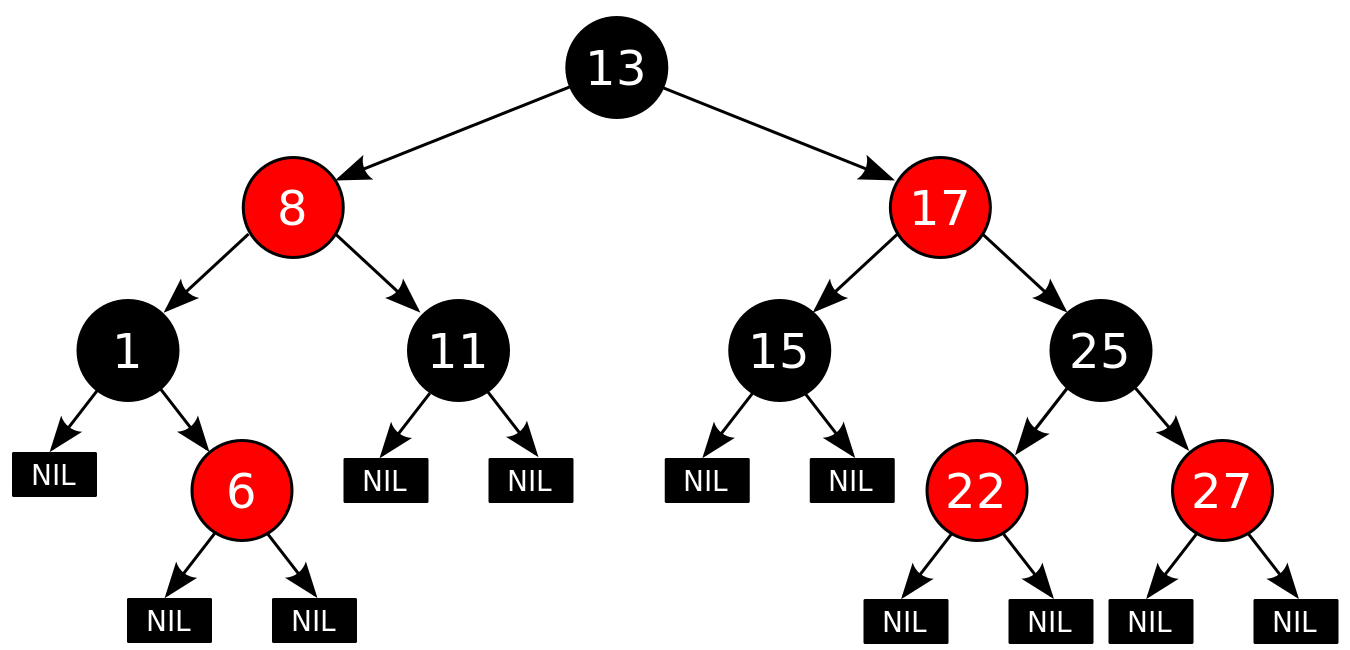
\includegraphics[width=\textwidth]{images/rbtree}};

      \tikz[align=left] \node [below=of rbtree,node font=\tiny\itshape] {By Cburnett -- Own work, CC
        BY-SA 3.0\\https://commons.wikimedia.org/w/index.php?curid=1508398};
    \end{column}

    \begin{column}{.5\textwidth}<3->
      \setlength{\bytesize}{0.2cm}
      \setlength{\memwidth}{8\bytesize}
      \setlength{\memheight}{5cm}

      \begin{tikzpicture}[
          word/.style={
            draw=black!50,
            minimum height=\bytesize,
            minimum width=8\bytesize,
            inner sep=0pt
          },
          anchor=south west
        ]

        \node (word) at (0,0) [word,fill=blue!90!black,text=white] {\tiny value};
        \node (next) [word,above=0 of word,fill=red!90!black] {};
        \node (prev) [word,above=0 of next,fill=yellow!90!black] {};
        \node (parent) [word,above=0 of prev,fill=green!90!black] {};
        \node (color) [word,above=0 of parent,fill=black!20!white] {};
        \node [above left=0 and -\bytesize of parent,
          rectangle,
          inner sep=0pt,
          minimum width=\bytesize,
          minimum height=\bytesize,
          draw=black!50,
          fill=none,
          label={90:{\tiny color}}
        ] {};

        \node (wordp) [word,above right=1.1 and .1 of word,fill=blue!90!black,opacity=.3] {};
        \node (nextp) [word,above=0 of wordp,fill=red!90!black,opacity=.3] {};
        \node (prevp) [word,above=0 of nextp,fill=yellow!90!black,opacity=.3] {};
        \node (parentp) [word,above=0 of prevp,fill=green!90!black,opacity=.3] {};
        \node (colorp) [word,above=0 of parentp,fill=black!20!white,opacity=.3] {};

        \node (wordl) [word,below left=1.1 and .1 of word,fill=blue!90!black,opacity=.3] {};
        \node (nextl) [word,above=0 of wordl,fill=red!90!black,opacity=.3] {};
        \node (prevl) [word,above=0 of nextl,fill=yellow!90!black,opacity=.3] {};
        \node (parentl) [word,above=0 of prevl,fill=green!90!black,opacity=.3] {};
        \node (colorl) [word,above=0 of parentl,fill=black!20!white,opacity=.3] {};

        \node (wordr) [word,below right=1.1 and .1 of word,fill=blue!90!black,opacity=.3] {};
        \node (nextr) [word,above=0 of wordr,fill=red!90!black,opacity=.3] {};
        \node (prevr) [word,above=0 of nextr,fill=yellow!90!black,opacity=.3] {};
        \node (parentr) [word,above=0 of prevr,fill=green!90!black,opacity=.3] {};
        \node (colorr) [word,above=0 of parentr,fill=black!20!white,opacity=.3] {};

        \draw[{Circle[length=2pt]}-Stealth,black!80] (parent.east) to [out=0,in=270] node[auto,swap] {\tiny parent} (wordp.south);
        \draw[{Circle[length=2pt]}-Stealth,black!80] (prev.west) to [out=180,in=90] node[auto,swap] {\tiny left} (colorl.north);
        \draw[{Circle[length=2pt]}-Stealth,black!80] (next.east) to [out=0,in=90] node[auto,swap] {\tiny right} (colorr.north);

      \end{tikzpicture}
    \end{column}
  \end{columns}
\end{frame}
